\section{What is the craziest thing that has happened to you?}
One of the craziest things that happened to me was nearly deadly.
In June 1967 I was 14 and participated with the youth group from church.
To help make the group larger we joined with the youth from a nearby church.

On this summer evening we were hosting a fundraising car wash.
We were working at two locations.
When the group I was with finished washing cars at our location we decided to join the other group.
We did not fit into the one car and so some of us decided to ride on the back of the car.
I ended up in the center of the car's trunk.

All went well until we were pulling out from a stop sign.
The driver decided to give us a bit of a thrill and started out rather quickly.
I had no place to hold in and realized that I was sliding off of the car.
I remember thinking that perhaps I could land on my feet, but alas we were going too fast.
I hit the ground.
Details after this were sketchy.
The ambulance was called.
I remember telling someone that our family doctor was Doctor Mustard, but then realized that he was no longer living.
I knew I was traveling in the ambulance.
\begin{figure}
\centering
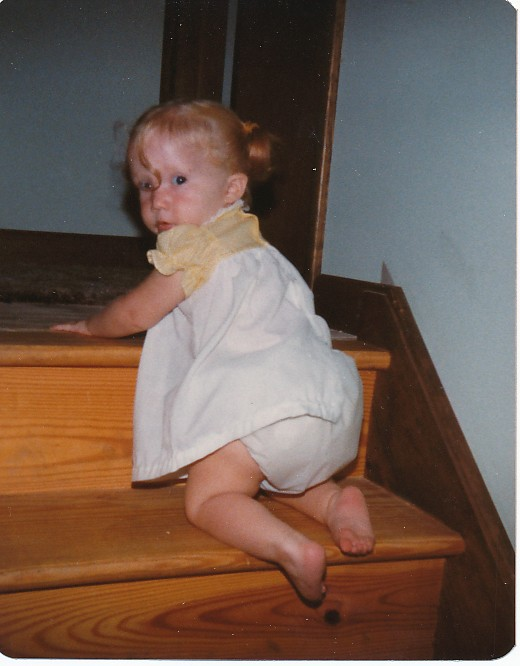
\includegraphics[width=0.9\textwidth]{childhood/11.jpg}
\caption{
Picture by Aunt Dorothy and clipping from the newspaper.
}
\end{figure}

From others I learned later that in the emergency room I appeared conscience and was talking.
When my parents arrived I was preparing to be discharged.
It was then that I went into convulsions.
I'm told that our church bishop was called and I was kept in the hospital.
This happened on a Wednesday evening.
I remember waking up in a darkened room.
I believe it was Friday morning and I was alone.
At first I did not know where I was and felt uncertain about what had happened.
I believe that I went home on Saturday.
